\documentclass[12pt,a4paper]{article}
\usepackage[utf8]{inputenc}
\usepackage[spanish]{babel}
\usepackage{amsmath}
\usepackage{amsfonts}
\usepackage{amssymb}
\usepackage{makeidx}
\usepackage{graphicx}
\usepackage{multicol}
\usepackage{changepage}
\usepackage{float}
\usepackage{cite}
\usepackage{url}
\usepackage[left=2cm,right=2cm,top=2cm,bottom=2cm]{geometry}

\title{PROYECTO NORMA ISO 9001}
\author{*Chiriguaya Alvaro, *Mite Lady, *Zambrano Allison}
\date{4 de marzo del 2020}
\begin{document}
%encabezado 
\pagestyle{plain}{
\pagestyle{empty}
\changepage{3cm}{1cm}{-0.5cm}{-0.5cm}{}{-2cm}{}{}{}
\noindent
  {\small
\begin{tabular}{p{0.75\textwidth} p{0.25\textwidth} }

\includegraphics[scale=0.3]{../../../Downloads/logoUniversidad.png}  &
\includegraphics[scale=0.5]{../../../Downloads/images.jpg} 
\end{tabular}
}
%datos de la caratula
\begin{center}
\par\vspace{2cm} %Rspacoo dejado antes del encabezado
{
\Huge\textbf{
Universidad de Guayaquil \\*[0.40cm] Facultad de Ciencias Matem\'aticas y F\'isicas}
}
\par\vspace{3cm}
{

\Large\textbf{Proyecto basado en la norma ISO 9001:20152}
\par\vspace{1cm}
\Large\textbf{Ingenier\'ia de Software}
\par\vspace{1cm}
\Large\textbf{Materia: Procesos de Software}
\par\vspace{1cm}
\Large\textbf{Docente: Ing. Miguel \'Angel Botto Tobar }
}
\par\vspace{2cm}
\large\textbf{ 4/03/2020}
\par\vspace{0.5cm}
\large\textbf{2019-2020} 
\par\vspace{3cm} 

\end{center}
\clearpage
}
\section{Normas ISO 9001}
La Norma ISO 9001:2015 es la base del Sistema de Gestión de la Calidad - SGC. Es una norma internacional que se centra en todos los elementos de la gestión de la calidad con los que una empresa debe contar para tener un sistema efectivo que le permita administrar y mejorar la calidad de sus productos o servicios. 
Los clientes se inclinan por los proveedores que cuentan con esta acreditación porque de este modo se aseguran de que la empresa seleccionada disponga de un buen SGC.

\section{Caso de estudio}
El TPV o POS (Point of Sale) es la evolución del siglo XXI de la clásica caja registradora. En el mundo de la hostelería y venta al por menor de pequeños comercios los TPV son utilizados para registrar ventas, beneficios, pedidos, inventarios, historial de clientes, etc. En resumen, un TPV otorga control sobre las operaciones de negocio.\\
Un TPV básico consiste en una computadora, un cajón de dinero, una impresora de tiques, un monitor y dispositivos de lectura como lector de códigos de barras, teclados, etc. Los TPV registran las transacciones y permiten generar detallados informes, permitiendo tomar mejores decisiones comerciales. El TPV correcto permitirá mejorar la productividad y redundará en mejores ganancias.\\
Un TPV puede revolucionar el funcionamiento de un comercio. Desde incrementar la productividad de los empleados hasta conocer si las inversiones obtienen beneficios.\\\\
\begin{center}
\includegraphics[width=0.6\textwidth]{../../../Downloads/01.jpg} 
\end{center}

\section{Sistema de gestion de calidad}
\subsection{Objeto y campo de aplicación}
Elaboración de un programa que sea ideal para la venta de comidas rápidas (pizzerias, hamburgueserias, bocadillerías, etc.). En donde se permita lo siguiente:
\begin{itemize}
\item Registra los datos del cliente.
\item Realizar pedidos a domicilio.
\item Gestiona los consumos de los clientes en el propio local.
\item Opción a que el cliente pueda el pedido telefónicamente y en lugar de servirle al domicilio viene a recogerlo al local.
\item Atención de pedidos en las mesas del local, de forma directa.
\item Permitir imprimir los listados para gestionar los temas del negocio. Entre otros: presupuestos, facturas realizadas, gastos, beneficios, listados de impuestos, etc.
\end{itemize}

\section{Referencias normativas}
ISO 9001: 2015, Sistemas de gestión de calidad. Fundamentos y vocabulario.

\section{Términos y definiciones}
Para los fines de este documento, aplican los términos y definiciones incluidos en la norma ISO 9001:2015 y los de la empresa especialista en la creación y venta de software “TPV Gratuito 123”.
\begin{center}
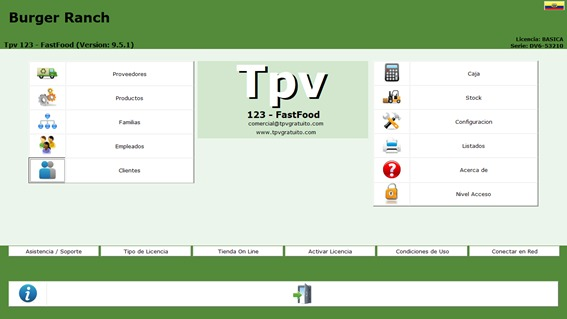
\includegraphics[width=0.9\textwidth]{../../../Downloads/1.jpeg}  
\end{center}

\section{Contexto de la organización}
El objetivo de la empresa es ayudar a los clientes a ahorrar tiempo y dinero en las gestiones diarias de su negocio, proporcionando sencillez y fiabilidad en sus gestiones, permitiéndoles concentrarse en la lógica de su negocio.
Se esfuerzan en introducir nuevas e interesantes características en nuestros productos.
Escuchan las peticiones de nuestros clientes para adaptar nuestras soluciones y satisfacer el mercado.
 Los TPV de la empresa son ampliamente utilizados por cientos de empresas en el mundo.
 Las opciones más necesarias y básicas son gratuitas.
 Dan cobertura a prácticamente todo tipo de negocios.
 Soporte técnico especializado en atender tus dudas e incidencias.
 
\subsection{Determinación del alcance}
El programa es ideal si el negocio de restaurante está orientado a Comida Rápida o también con el conocido término de FastFood. Es decir que podrá ser implementado en restaurantes como:
\begin{itemize}
\item Pizzerías
\item Hamburgueserías
\item Bocadillerías
\item Taquerías\\\\
\end{itemize}

\subsection{Procesos}
El programa cuenta con los siguientes procesos:
Pedidos a domicilio.
\begin{itemize}
\item Consumo en local.
\item Pedido telefónico y recogida en local.
\item Servicio en mesa.
\item Caja.
\item Listados.\\\\
\end{itemize}

\subsection{Liderazgo}
\subsection{Planificación}
\subsection{Apoyo}
\subsection{Operación}
\subsection{Evaluación del desempeño}
\subsection{Mejora}

\subsection{Diseño y desarrollo}
Abordamos la interpretación y aplicación de los requisitos del diseño y desarrollo de productos y servicios según la norma ISO 9001  
Nuestro programa incluye la materializacion de resultados de un diseño aprobado asi logrando la atracción y desrrollo de nuevos productos y servicios. El diseño y desarrollo implica crear o determinar como debe ser algo que satisface los requisitos. El diseño y desarrollo se basa en las necesidades del cliente, todos los requisitos deben llevar a cabo. El sistema cuenta con un un panel para la selección del empleado, cliente que va a solicitar el producto y asegura a cierta información de la empresa.\\\\

\subsection{Validación del diseño y desarrollo}
En la fase de validación del diseño y desarrollo e las normas ISO 9001, se  debe ralizar una revisión como está avanzando el diseño de nuestro producto o servicio. Verificamos para ver si efectivamente lo que hemos estado haciendo cumple con los elementos de entrada. Las verificaciones se establecen en la planificación del proyecto y la realizamos cuando podemos comparar una variable de nuestro diseño con los elementos de entrada. Validamos el funcionamiento de nuestro diseño. Dicho de otra forma, nos aseguramos si el producto o servicio sirve o no para cumplir su cometido.
\end{document}